\chapter{Contributors}

%~ \setlength{\columnseprule}{1pt}

\begin{multicols}{2}

   
\begin{wrapfigure}{l}{3.3cm}

\vspace{-5pt}

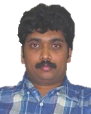
\includegraphics[scale=4.2]{src/Figures/authors/Rajavelsamy.png}

 \vspace{-8pt}

\end{wrapfigure}    

\textbf{Rajavelsamy R} is an Architect (General Manager) in the Standards Team of Samsung R\&D Institute India, Bengaluru. He received Bachelor of Engineering Degree in Electronics and Communication Engineering and Master of Technology Degree in Computer Science and Engineering. He joined Samsung Electronics, at its India office in 2003 and has been with its Standards Team, focusing on research and standardization of wireless mobile communications. He has 15+ years of rich experience in Security system architectures, Security protocols, Wireless cellular communications systems and protocols, where he has contributed in research and standardization of Samsung Telecommunication products. Since 2004, he has been actively involved in contributing and participating in 3GPP SA3 meetings representing Samsung. He has actively contributed since Rel-6, e.g. WCDMA, IWLAN, H(e)NB, LTE, MTC, ProSe, MCX, CAPIF, 5G standardization. He also served as Vice Chairman of 3GPP SA3 WG (July 2007 to Nov 2009). He is active as rapporteur for several 3GPP SA3 work items specifically, MTC, CAPIF, IAB, SCAS-UPF.

\vskip -.5cm

\dotfill 

\vskip -.4cm

    \begin{wrapfigure}{l}{3.3cm}

\vspace{-12pt}

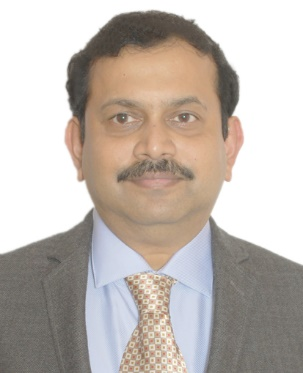
\includegraphics[scale=.3]{src/Figures/authors/D-Das.png}

\vspace{-10pt}

\end{wrapfigure}
    
\textbf{Prof.~Debabrata Das} is Professor at IIIT-Bengaluru (IIIT-B). Before joining IIIT-B, he had served at G S Sanyal School of Telecommunication at IIT Kharagpur and later at Kirana Networks in New Jersey, USA. At present, he is Principal Investigator (PI) of projects from Department of Electronics and Information Technology, Government of India on Green Broadband Wireless Network and Nokia Research on IoT. He was PI of sponsored projects from Intel, Hewlett Packard, Microsoft, Motorola Research, Nokia, Govt. of India on areas of IMS and Broadband Wireless MAC/QoS/Energy-saving, TVWS and Security. He has more than 125 peer reviewed papers in different journals and International conferences. He has 1 accepted US patent and 10 more are under review. Dr. Das received his Ph.D. degree from IIT-Kharagpur and MTech from IIT-Varanasi. He is a Board Member of IIIT-Bhubaneswar; Technical and Empower Committee member of e-Governance, Govt. of Karnataka. He is Fellow of Institution of Electronics \& Telecommunication Engineers (IETE) and Fellow-IE. He Das is recipient of Global IEEE MGA Achievement Award 2012 and Prof.~K Sreenivasan memorial outstanding teaching award in the areas of Electronics and Telecommunication in 2017.    

\vskip -.5cm

\dotfill 

\vskip -.4cm

\begin{wrapfigure}{l}{3.2cm}
\vspace{-12pt}

\includegraphics[scale=.052]{src/Figures/authors/NBhat.png}

\vspace{-9.5pt}
\end{wrapfigure}

\textbf{Prof.~Navakanta Bhat} received his B.E. in Electronics and Communication from SJCE, University of Mysore in 1989, M.Tech. in Microelectronics from I.I.T. Bombay in 1992 and Ph.D. in Electrical Engineering from Stanford University, Stanford, CA in 1996. Then he worked at Motorola’s Networking and Computing Systems Group under Advanced Products R\&D Lab (APRDL)  in Austin, TX until 1999. At Motorola he worked on logic technology development and he was responsible for developing high performance transistor design and dual gate oxide technology for PowerPC microprocessors. He joined the Indian Institute of Science, Bengaluru in 1999 where he is currently a Professor and Chair, Centre for Nano Science and Engineering. His current research is focused on Nanoelectronics device technology, Biosensors for point of care diagnostics and Gas sensors for pollution monitoring. He has 250 research publications in international journals and conferences and 10 granted US patents and 14 pending patents to his credit. He was instrumental in creating the National Nanofabrication Centre (NNfC) at IISc, Bengaluru, benchmarked against the best university facilities in the world. He served as the chairman of NNfC administration committee (2010 – 2015).

 %~ \vskip -.1cm

He is an elected Fellow of the Indian National Academy of Engineering and elected Fellow of IEEE. He has received the Young Engineer Award (2003) from the Indian National Academy of Engineering, Swarnajayanti fellowship (2005) from the Department of Science and Technology, Govt. of India and Prof. Satish Dhavan award (2005) from the Govt. of Karnataka. He is also the recipient of IBM Faculty award 2007 and Outstanding Research Investigator award (2010) from DAE. For his translational research work, he has received Dr. Abdul Kalam Technology Innovation National Fellowship (2018), Prof. Rustum Choksi award for Excellence in Engineering Research (2017), Nina Saxena Technology Excellence award (2018), NASI Reliance Industries Platinum Jubilee award (2018) and BIRAC Innovator award (2018). He has also received the prestigious Infosys Prize (2018) for his contributions in Engineering and Computer Science category. 

\vskip -.2cm

He is currently (2016-2019) a member of the Board of Governors of the IEEE Electron Devices Society and also the Chair of Nanotechnology technical committee. He was the Editor of IEEE Transactions on Electron Devices, (2013-2015),  and the chief-editor of the IEEE TED special issue on “2D Materials for Electronic, Optoelectronic and Sensors”. He was the founding chair of the IEEE Electron Devices and Solid-State Circuits society, Bengaluru chapter which was recognized as the Outstanding Chapter of the Year by the IEEE SSC society (2003) and IEEE EDS society (2005). He was the technical program chair for the International Conference on VLSI design and Embedded Systems (2007) and co-General chair of the International conference on Emerging Electronics (2012). He is a Distinguished Lecturer of the IEEE Electron Devices Society.

\vskip -.5cm

\dotfill 

\vskip -.3cm 

\begin{wrapfigure}{l}{3.3cm}
\vspace{-12pt}

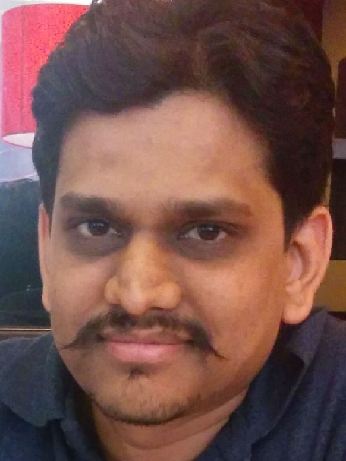
\includegraphics[scale=1.1]{src/Figures/authors/SanjeevG.png}

\vspace{-9.5pt}
\end{wrapfigure}

\textbf{Prof.~Sanjeev Gurugopinath} received B.~E.~degree in Electrical and Electronics Engineering from Dr.~Ambedkar Institute of Technology, Visvesvaraya Technological University, Bengaluru, in 2004, the M.~Tech.~degree in Digital Electronics and Communication Engineering from  M.~S.~Ramaiah Institute of Technology, Visvesvaraya Technological University, Bengaluru, in 2006, and  Ph.D. in signal processing for communications from the Indian Institute of Science, Bengaluru, in 2015. He is currently a Professor with the Department of Electronics and Communication Engineering, PES University, Bengaluru. His research interests are in the areas of cognitive radios and heterogeneous networks for 5G communication systems, powerline communications, underwater acoustics, and speech signal processing. He was a co-recipient of the Best Paper Award across all tracks at IEEE INDICON 2016. He is a member of IEEE, and a life member of ACCS.

\vskip -.5cm

\dotfill 

\vskip -.3cm

\begin{wrapfigure}{l}{3.2cm}
\vspace{-12pt}

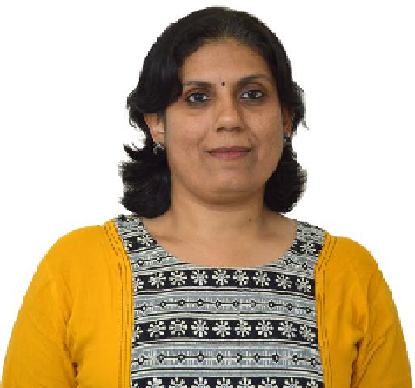
\includegraphics[scale=.9]{src/Figures/authors/Aparna-Gooru-Lab.png}

\vspace{-12pt}
\end{wrapfigure}

\textbf{Dr.~Aparna Lalingkar}, before joining Gooru labs, was a postdoctorate research fellow at University of Haifa, Israel under the fellowship of Planning and Budgeting Commission of Israeli Higher Education.

\vskip -.3cm

She is a mathematician and educational technologist with PhD in Information Technology. For PhD she had proposed an ontology for teaching problem solving in mathematics. Her research interest include: application of Information Technology to Education specifically mathematics and science education, application of semantic web technology to education, ontological engineering and management, online assessment, automation of applications, educational technology and management.

\vskip -.2cm

She earned an MPhil in math education research from Cambridge University, UK and have received several academic fellowships and awards including HP Labs fellowship for PhD, DFID \& CCT fellowship for MPhil.

\vskip -.2cm

She has wide range of teaching and work experience. She has taught tribal students as well as intellectually gifted students. She has also taught graduate level and master’s level students. During PhD at IIITB, she has mentored MTech students for some projects.

\vskip -.5cm

\dotfill 

\vskip -.3cm  


\begin{wrapfigure}{l}{3.2cm}
\vspace{-12pt}

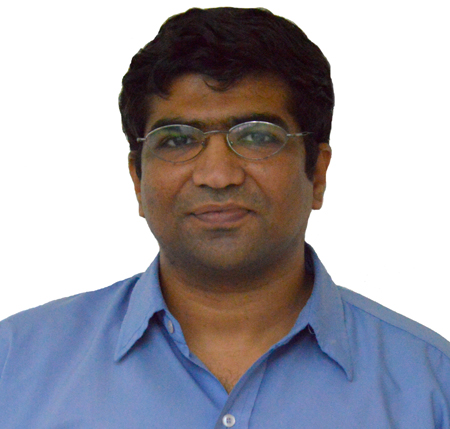
\includegraphics[scale=.8]{src/Figures/authors/srinath_srinivasa.png}

\vspace{-9pt}
\end{wrapfigure}

\textbf{Prof.~Srinath Srinivasa} heads the Web Science lab and is the Dean (R\&D) at IIIT Bangalore, India. Srinath holds a Ph.D. (magna cum laude) from the Berlin Brandenburg Graduate School for Distributed Information Systems (GkVI) Germany. He holds an M.S. (by Research) degree from IIT-Madras and a B.E. degree in Computer Science and Engineering from The National Institute of Engineering (NIE) Mysore. He works in the area of Web Science — that models of the impact of the web on humanity. Technology for educational outreach and social empowerment has been a primary motivation driving his research. He has participated in several initiatives for technology-enhanced education including the VTU Edusat program, The National Programme for Technology Enhanced Learning (NPTEL) and an educational outreach program in collaboration with Upgrade.

\vskip -.3cm 

He is a member of various technical and organizational committees for international conferences like International Conference on Weblogs and Social Media (ICWSM), ACM Hypertext, COMAD/CoDS, ODBASE, etc. He is also a life member of the Computer Society of India (CSI). As part of academic community outreach, Srinath has served on the Board of Studies of Goa University and as a member of the Academic Council of the National Institute of Engineering, Mysore. He has served as a technical reviewer for various journals like the VLDB journal, IEEE Transactions on Knowledge and Data Engineering, and IEEE Transactions on Cloud Computing. He is also the recipient of various national and international grants for his research activities.

\vskip -.5cm

\dotfill 

\vskip -.3cm 

\begin{wrapfigure}{l}{3.2cm}
\vspace{-12pt}

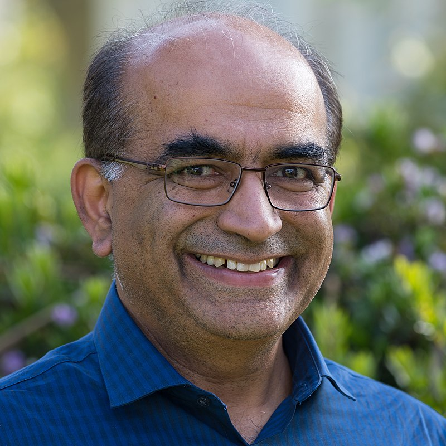
\includegraphics[scale=.82]{src/Figures/authors/Prasad_Ram,_June_2019.png}

\vspace{-6.5pt}

\end{wrapfigure}

\textbf{Prasad Ram} (aka Pram) is the Founder, CEO and Chairman of Gooru. While working at Google, Pram devised a prototype to address his problem of finding age and topic appropriate educational resources on the web. Gooru, as it is today, began as a “20\%\break effort” evolved into a year-long pilot in India that included 1,000 students across 25 classrooms. Pram left Google to pursue Gooru as a not-for-profit education technology start-up. Pram has previously worked at Xerox Research, Dynamx Technology (co-founder), Yahoo! and Google. Pram has a Ph.D. and M.S. in Computer Science from UCLA, and he obtained his B.Tech. in Computer Science from IIT-Bombay. You can reach Pram at pram@gooru.org.


\vskip -.4cm

\dotfill 

\vskip -.3cm  

\begin{wrapfigure}{l}{3.1cm}
\vspace{-12pt}

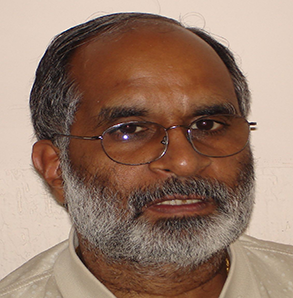
\includegraphics[scale=.9]{src/Figures/authors/Rustagi_RPR-PP-Photo.png}

\vspace{-6pt}
\end{wrapfigure}

\textbf{Prof.~Ram P. Rustagi} is currently working as Professor, CSE dept, KSIT Bangalore, and honed up his academic skills with Ph.D from IIT Delhi, and M.Tech from IISc Bangalore. Prior to KSIT, at Cavisson Systems, he mentored new technology development using Machine Learning techniques in Security and Performance Monitoring. At PES University, he had taught Undergraduates, Post Graduates students, and successfully guided 3 Ph.D scholars. At PESU, he brought innovations in teaching computer network and security courses, and introduced practical experiential learning exercises.

\vskip -.4cm

\dotfill 

\vskip -.3cm  

\begin{wrapfigure}{l}{3.2cm}
\vspace{-12pt}

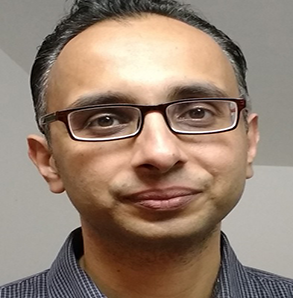
\includegraphics[scale=1]{src/Figures/authors/Viraj_Kumar.png}

\vspace{-5pt}
\end{wrapfigure}

\textbf{Prof.~Viraj Kumar} is a Visiting Professor at the Divecha Centre for Climate Change, IISc Bangalore and the Vice-Chair of ACM India’s Special Interest Group in Computer Science Education (iSIGCSE). He was a consultant to the Committee to draft the National Education Policy (2017-18), and contributed to two education-related task groups of the Karnataka Knowledge Commission (2014-16). He holds a PhD in Computer Science from the University of Illinois at Urbana-Champaign.

\end{multicols}

